\documentclass[handout,aspectratio=169]{beamer}
\usepackage{graphicx}
\usepackage{booktabs}
\usepackage{array}
\usepackage{listings}
\usepackage{xcolor}

\definecolor{codegreen}{rgb}{0,0.6,0}
\definecolor{codegray}{rgb}{0.5,0.5,0.5}
\definecolor{codepurple}{rgb}{0.58,0,0.82}
\definecolor{backcolour}{rgb}{0.95,0.95,0.92}

\lstset{
    backgroundcolor=\color{backcolour},
    commentstyle=\color{codegreen},
    keywordstyle=\color{magenta},
    numberstyle=\tiny\color{codegray},
    stringstyle=\color{codepurple},
    basicstyle=\ttfamily\scriptsize,
    breakatwhitespace=false,
    breaklines=true,
    captionpos=b,
    keepspaces=true,
    numbers=left,
    numbersep=5pt,
    showspaces=false,
    showstringspaces=false,
    showtabs=false,
    tabsize=2
}

\title{Re-processing Perturb-Seq datasets from FASTQ}
\subtitle{First Results for the Unified Pipeline}
\date{2026-04-28}
\author{Kirill Tsukanov \\ Senior Full Stack Developer \& Data Engineer \\ \texttt{ktsukanov@ebi.ac.uk}}
\institute{All Hands Meeting}

\setbeamertemplate{navigation symbols}{}
\setbeamertemplate{footline}{%
  \begin{beamercolorbox}[wd=\paperwidth,ht=2.5ex,dp=1.5ex,center]{}
    \hspace{15pt}\usebeamerfont{author in head/foot}Unified FASTQ Re-analysis Pipeline
    \hfill
    \usebeamerfont{date in head/foot}\insertframenumber{} / \inserttotalframenumber
    \hspace{15pt}
  \end{beamercolorbox}%
}

\begin{document}

\begin{frame}
    \titlepage
\end{frame}

\begin{frame}{Why re-process from FASTQ?}
    \begin{itemize}
        \item \textbf{Consistency:} scPerturb datasets are usually deposited as processed H5AD files, but they come from different pipelines, references, and filtering choices.
        \item \textbf{Comparable outputs:} Re-processing gives us a common count matrix layout, common metadata expectations, and a consistent way to attach guide counts.
        \item \textbf{Quality control:} Raw reads let us apply the same checks across studies instead of inheriting every author-specific decision.
        \item \textbf{Catalogue expectation:} Users expect harmonised data in the Perturbation Catalogue, not only links to heterogeneous processed files.
    \end{itemize}
\end{frame}

\begin{frame}{Why Kallisto + Bustools?}
    \begin{itemize}
        \item \textbf{Speed:} Kallisto + Bustools is much faster than Cell Ranger while giving very comparable expression quantification.
        \item \textbf{Resource fit:} We have adequate, but not unlimited, compute and storage. The pipeline must work within those limits.
        \item \textbf{Full catalogue scale:} We want to process all datasets we have, and be able to reprocess them if the pipeline improves.
        \item \textbf{Future-proofing:} New perturb-seq datasets are expected to be very large, so the pipeline needs to scale well rather than depend on throwing more hardware at each run.
    \end{itemize}
\end{frame}

\begin{frame}{Pipeline Status}
    \begin{itemize}
        \item The unified FASTQ-to-H5AD pipeline is now implemented in Nextflow and runs on the EBI Slurm cluster with Singularity.
        \item The first full dataset has been processed end-to-end: Nadig 2025 Jurkat.
        \item The output is a single compressed \texttt{experiment\_final.h5ad}.
        \item Gene expression counts are stored in \texttt{.X}; guide counts are stored in \texttt{.obsm['guides']} with guide names in \texttt{.uns['guide\_names']}.
        \item Per-sample guide merge diagnostics are written next to the merged H5AD files.
    \end{itemize}
\end{frame}

\begin{frame}{Pipeline Architecture}
    \begin{enumerate}
        \item \textbf{Prepare samples:} Parse ENA metadata and group SRR runs by physical 10x well.
        \item \textbf{Build references:} Create cDNA and KITE guide indices from Ensembl GRCh38 and \texttt{features.tsv}.
        \item \textbf{Count reads:} Run \texttt{kb count} separately for mRNA and sgRNA FASTQs for each physical sample.
        \item \textbf{Merge modalities:} Align guide counts to filtered mRNA cell barcodes.
        \item \textbf{Concatenate samples:} Add sample-specific barcode suffixes and write one unified H5AD.
    \end{enumerate}
    \vspace{0.8em}
    \centering
    \textbf{Key design point:} sample-aware grouping prevents barcode collisions between separate physical wells.
\end{frame}

\begin{frame}{Development Issues Solved}
    \begin{itemize}
        \item \textbf{ENA FASTQs missing technical reads:} Historical ENA FASTQs for this dataset do not include the barcode/UMI reads. Current workaround: SRA download with technical reads included. We notified ENA; they are aware and plan to fix it, so future runs may use ENA directly.
        \item \textbf{Sample grouping:} SRRs and lanes must be grouped by physical well before counting. This is currently parsed from ENA library names; later versions may autodetect this.
        \item \textbf{Barcode collisions:} Final concatenation adds sample suffixes so identical 10x barcodes from different wells remain distinct.
        \item \textbf{GEX/KITE matching:} Guide barcodes are not exactly the same as expression barcodes in this dataset. The pipeline applies the required KITE barcode correction before alignment.
    \end{itemize}
\end{frame}

\begin{frame}[fragile]{Pipeline Execution}
\begin{lstlisting}[language=bash]
nextflow run main.nf \
  -profile slurm,singularity \
  --fastq_dir $HPS_PATH/perturb_seq_fastq/SAMN40972597 \
  --metadata_tsv $HPS_PATH/perturb_seq_fastq/SAMN40972597/ena_metadata.tsv \
  --outdir $HPS_PATH/perturb_seq_fastq/results \
  --chemistry 10xv3 \
  --transcriptome_fa $HPS_PATH/cache/reference/Homo_sapiens.GRCh38.dna.primary_assembly.fa.gz \
  --gtf $HPS_PATH/cache/reference/Homo_sapiens.GRCh38.111.gtf.gz \
  --features_tsv $HPS_PATH/perturb_seq_fastq/SAMN40972597/features.tsv
\end{lstlisting}
    \vspace{0.4em}
    \begin{itemize}
        \item The sample sheet is generated automatically from ENA metadata.
        \item mRNA and sgRNA workflows run in parallel per sample.
        \item Guide counts are merged from unfiltered KITE output, then aligned to filtered mRNA cells.
    \end{itemize}
\end{frame}

\begin{frame}{First Dataset: Nadig 2025 Jurkat}
    \begin{itemize}
        \item Processed from raw FASTQs into a unified H5AD.
        \item The comparison was run against the author-provided H5AD.
        \item Analysis compares shared cells and shared genes after barcode and gene-name alignment.
        \item The main question: does the reprocessed dataset preserve expression signal, and how many guide calls match the original labels?
    \end{itemize}
    \vspace{0.8em}
    \centering
    \textbf{Short answer:} expression alignment is excellent; guide recovery is currently limited by strict dual-probe calling.
\end{frame}

\begin{frame}{Expression Agreement: Summary}
    \centering
    \begin{tabular}{lccc}
        \toprule
        \textbf{Metric} & \textbf{Pearson} & \textbf{Spearman} & \textbf{Deviant cells/genes} \\
        \midrule
        Total UMI counts per cell & 0.9997 & 0.9995 & 60.18\% \\
        Detected genes per cell & 0.9999 & 0.9998 & 0.01\% \\
        Mean expression per gene & 0.9588 & 0.9523 & 13.39\% \\
        Gene dropout rate & 0.9598 & 0.9523 & 7.48\% \\
        \bottomrule
    \end{tabular}
    \vspace{1.0em}
    \begin{itemize}
        \item Cell-level expression structure is almost identical to the author-processed dataset.
        \item Median cell-wise expression correlation is 0.9597.
        \item The main total-count difference is scale, not loss of biological structure.
    \end{itemize}
\end{frame}

\begin{frame}{Cell-Level Expression Agreement}
    \begin{columns}[T,onlytextwidth]
        \begin{column}{0.49\textwidth}
            \centering
            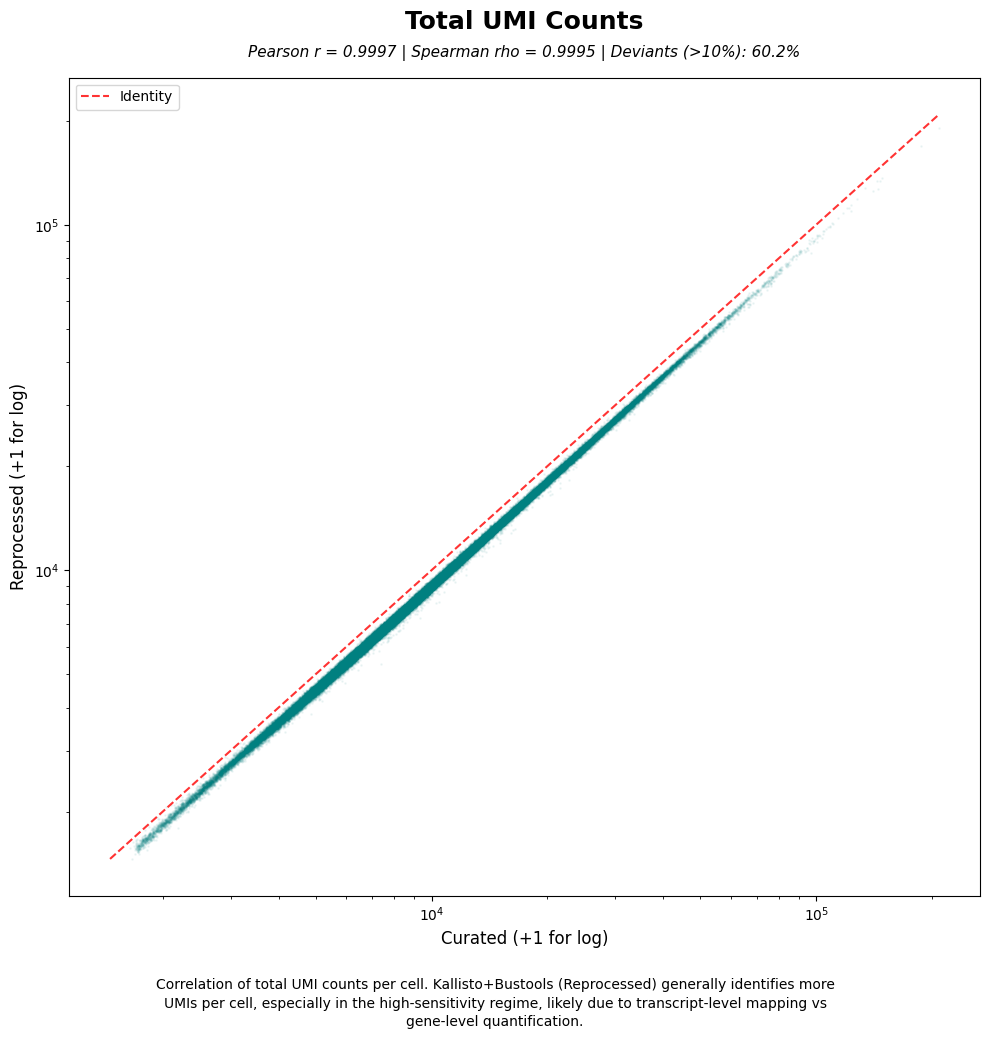
\includegraphics[width=\linewidth,height=0.72\textheight,keepaspectratio]{umi.png}

            \small Total UMI counts
        \end{column}
        \begin{column}{0.49\textwidth}
            \centering
            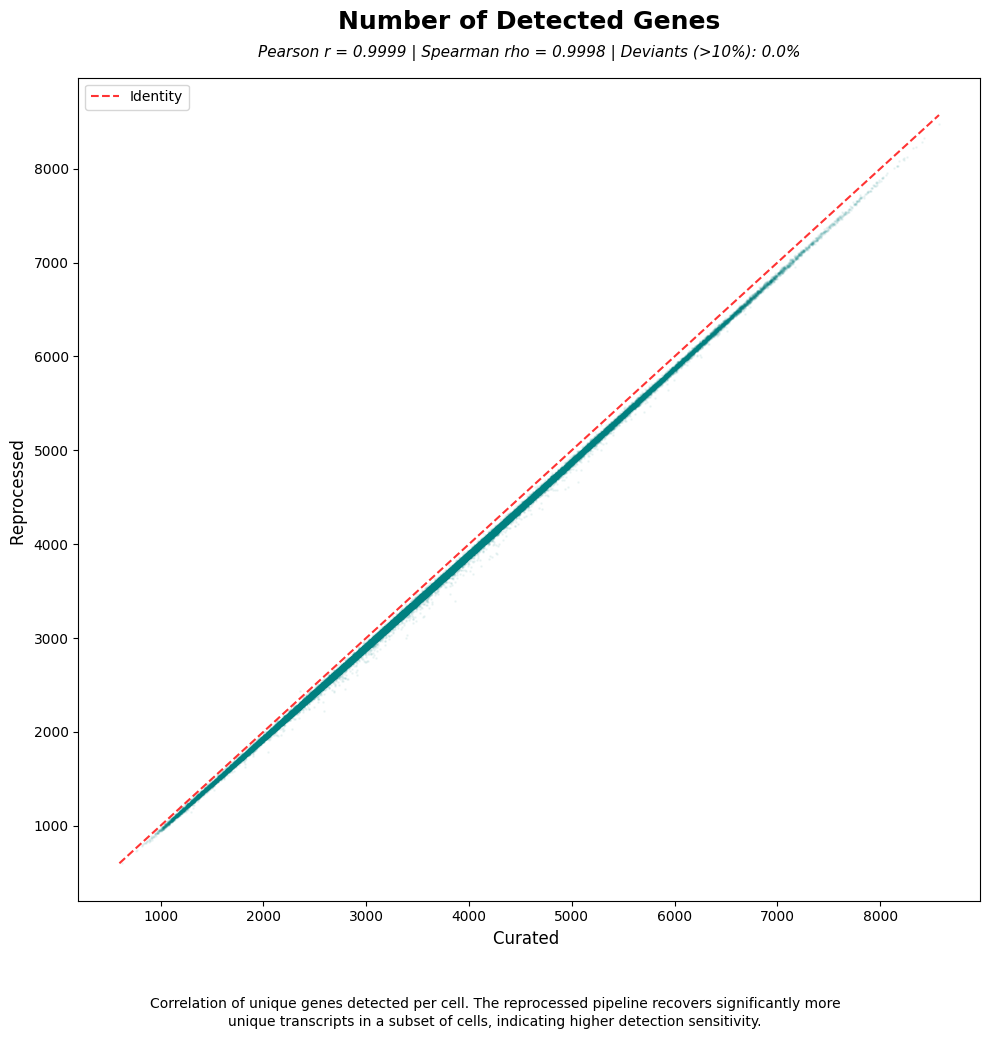
\includegraphics[width=\linewidth,height=0.72\textheight,keepaspectratio]{genes.png}

            \small Number of detected genes
        \end{column}
    \end{columns}
\end{frame}

\begin{frame}{Gene-Level Expression Agreement}
    \begin{columns}[T,onlytextwidth]
        \begin{column}{0.49\textwidth}
            \centering
            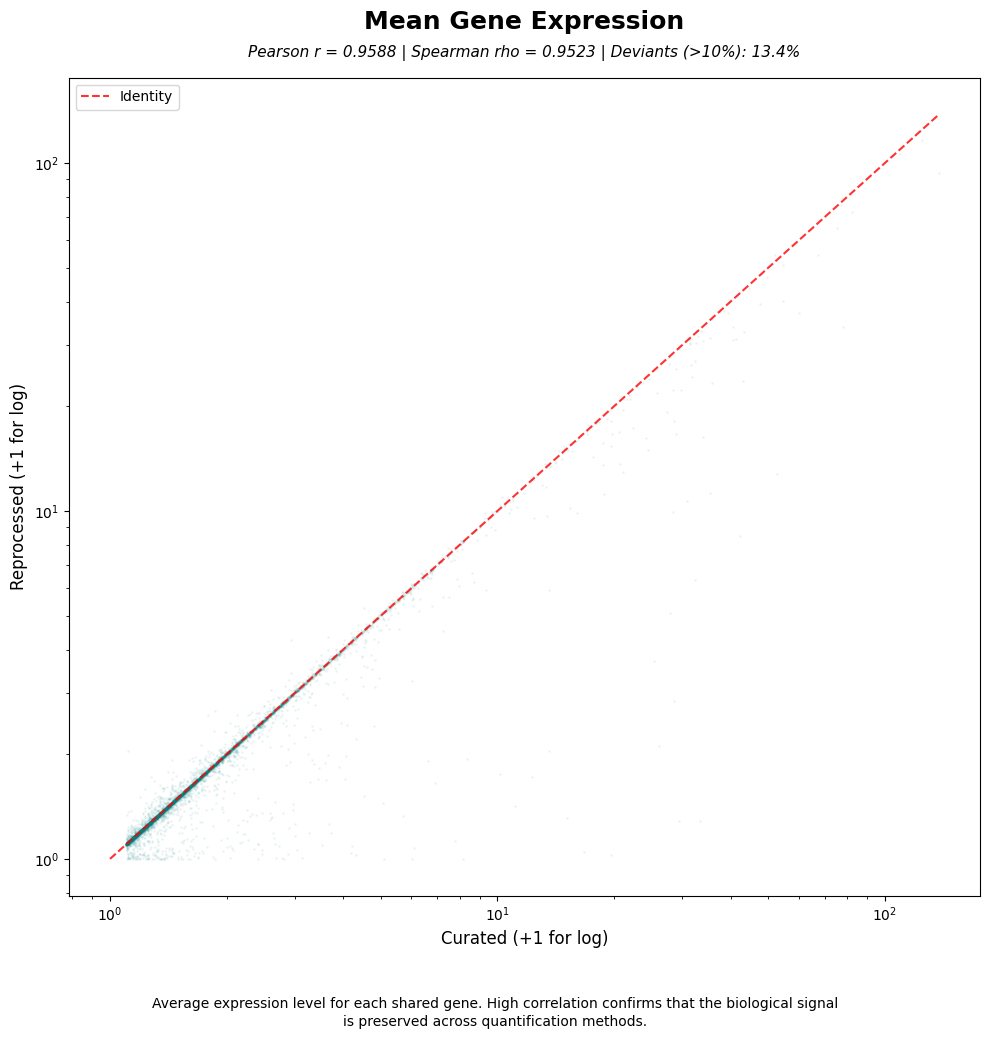
\includegraphics[width=\linewidth,height=0.72\textheight,keepaspectratio]{expression.png}

            \small Mean gene expression
        \end{column}
        \begin{column}{0.49\textwidth}
            \centering
            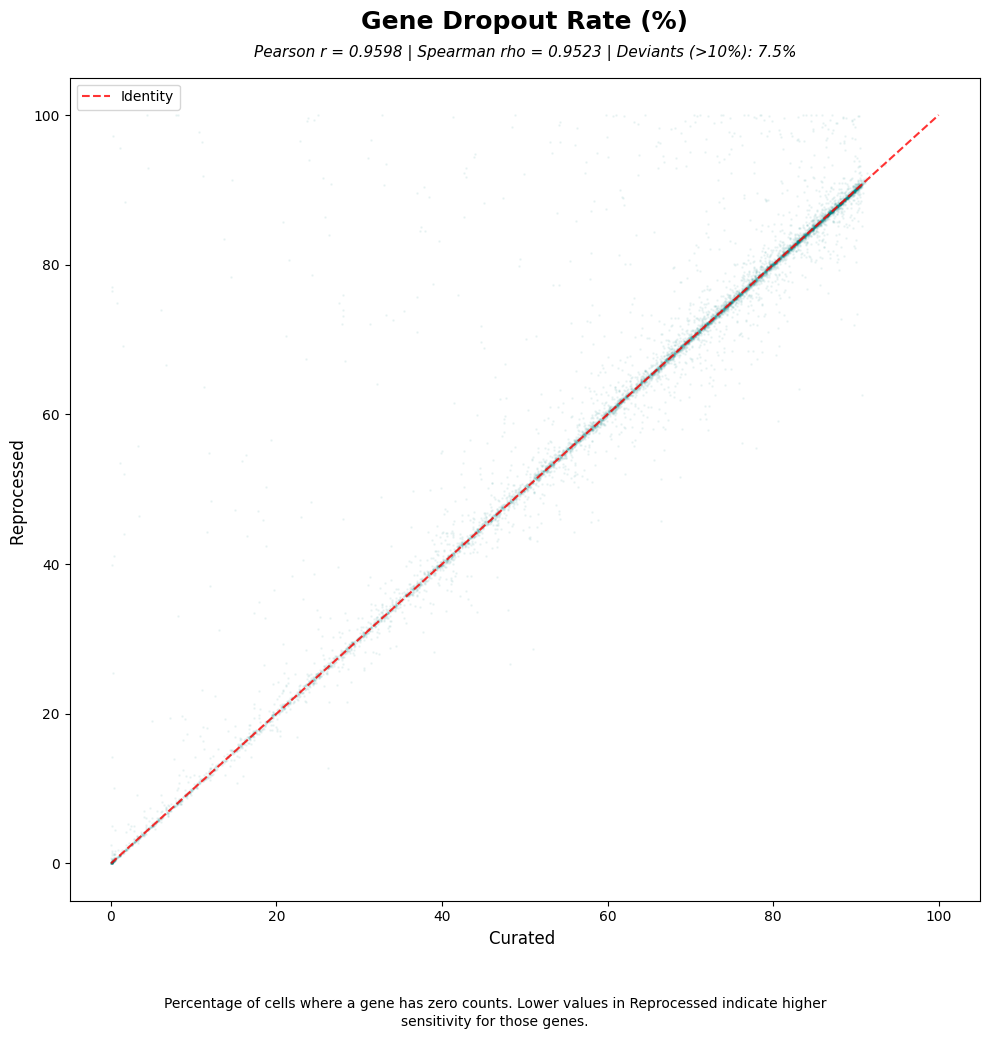
\includegraphics[width=\linewidth,height=0.72\textheight,keepaspectratio]{dropout.png}

            \small Gene dropout rate
        \end{column}
    \end{columns}
\end{frame}

\begin{frame}{Guide Recovery: Current Result}
    \begin{itemize}
        \item The comparison uses a strict guide call: two positive guides, both targeting the same gene, with at least 5 counts each.
        \item Under this rule, the reprocessed data recovers 164,757 of 214,522 curated dual-guide cells.
        \item Exact guide-pair agreement: \textbf{76.80\%}.
        \item Target-level agreement: \textbf{76.80\%}.
        \item The missing calls are mostly cells where only one of the two curated probes passes the 5-count threshold.
    \end{itemize}
    \vspace{0.8em}
    \centering
    \textbf{Interpretation:} current guide recovery is about threshold/calling behaviour, not a failure of the expression pipeline.
\end{frame}

\begin{frame}{Guide Signal Diagnostics}
    \centering
    \begin{tabular}{lrrr}
        \toprule
        \textbf{Threshold} & \textbf{Both curated probes} & \textbf{Exactly one probe} & \textbf{Neither probe} \\
        \midrule
        $\geq$ 1 count & 173,043 & 41,332 & 147 \\
        $\geq$ 2 counts & 170,245 & 44,038 & 239 \\
        $\geq$ 5 counts & 164,752 & 46,288 & 3,482 \\
        $\geq$ 10 counts & 158,854 & 47,254 & 8,414 \\
        \bottomrule
    \end{tabular}
    \vspace{1.0em}
    \begin{itemize}
        \item Across all reprocessed cells, 539,208 have at least one guide with 5+ counts.
        \item 487,177 have two or more guides with 5+ counts.
        \item 302,165 receive a dual same-target guide call before restricting to curated shared cells.
    \end{itemize}
\end{frame}

\begin{frame}{What We Have Now}
    \begin{itemize}
        \item A working, reproducible FASTQ-to-H5AD pipeline for perturb-seq datasets with GEX and guide modalities.
        \item A comparison workflow that checks cell-level expression, gene-level expression, dropout, and perturbation labels.
        \item First results showing very strong expression agreement with the author-processed data.
        \item A clear guide-calling question to tune next: how strict should dual-probe recovery be?
    \end{itemize}
\end{frame}

\begin{frame}{Next Steps}
    \begin{itemize}
        \item \textbf{Guide recovery:} Experiment with guide recovery settings. The current 5+5 threshold may be too strict.
        \item \textbf{Scale-out:} Run the pipeline on all available perturb-seq datasets.
        \item \textbf{Downstream analysis:} Run distance metrics between genes, plus the existing DEA and GSEA workflows.
    \end{itemize}
\end{frame}

\begin{frame}{Questions}
    \centering
    \Large Thank you
\end{frame}

\end{document}
